\chapter{Lecture 11}

This lecture is about \texttt{Multi-Way Models} where chapter \texttt{WireOverview.pdf} should be looked upon.

\begin{itemize}
  \item A brief history of multi-way analysis
  \item Tensor Nomenclature
  \item Tucker Decomposition
  \item CandeCom/PARAFAC (CP)
  \item Core Consistency Diagnostic
  \item Other tensor factorization models
  \item Missing values
  \item Software
  \item Applications
\end{itemize}

\section{Tensors}

Tensors, or multiway arrays, are generalizations of vectors (first-order tensors) and matrices (second-order tensors) to arrays of higher orders (N > 2). As such, a 3rd order tensor is an array with elements $x_{i,j,k} $

\begin{figure}[H]
  \centering
  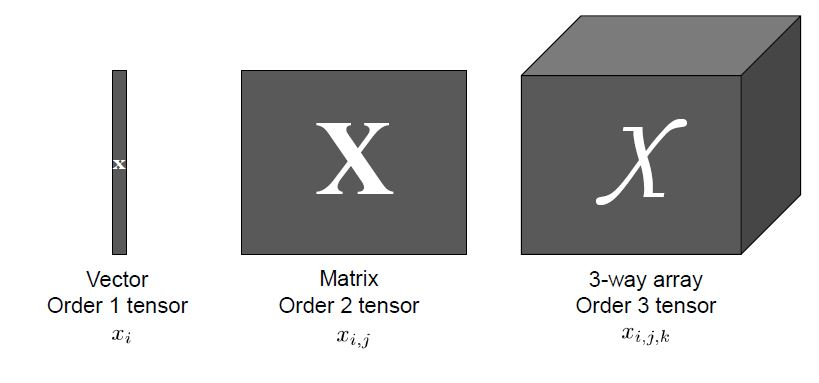
\includegraphics[width=0.9\textwidth]{tesnorexa}
  \caption{Tensor Example}\label{fig:tesnorexa}
\end{figure}

The reason to use tensor decomposition

\begin{itemize}
  \item Tensor decomposition admit uniqueness of the decomposition without additional constraints such as orthogonalityand independence
  \item Tensor decomposition methods can identify components even when facing very poor signal to noise ratios (SNR) and when only a relatively small fraction of all the data is observed.
  \item Tensor decomposition can explicitly take into account the multi-way structure of the data that would otherwise be lost when analyzing the data by collapsing some of the modes to form a matrix
\end{itemize}

The tensor vs matrix decomposition

Factorizing tensors have several advantages over two-way matrix

\begin{itemize}
  \item Uniqueness
  \item Component identification even when only a relatively small fraction of all the data is observed
  \item Multi-way decomposition techniques can explicitly take into account the multi-way structure of the data that would otherwise be lost when analyzing the data by matrix factorization approaches by collapsing some of the modes
\end{itemize}

However, factorizing tensors has its challenges

\begin{itemize}
  \item Its geometry is not yet fully understood
  \item The occurrence of so-called degenerate solutions
  \item Lack of guarantee of finding the optimal solution
\end{itemize}

\section{Tensor Nomenclature}

A general tensor of order $N$ is written

\[
    \mathcal{X} \in \mathbb{R}^{I_1 \times I_2 \times ... \times I_n}
\]

we will use the following notation to more compactly denote the size of a tensor

\[
    \mathcal{X}^{I_1 \times I_2 \times ... \times I_n}
\]

a given element of the tensor $\mathcal{X}$ is denoted by $x_{i_1, i_2, ..., i_N}$ from lecture \cite[p.~10]{lecture11}.

Consider the third order tensor $\mathcal{A}^{I \times J \times K}$ and $\mathcal{B}^{I \times J \times K}$. Scalar multiplication addition of two tensors and the inner product between two tensors are given by

\[
    \alpha \mathcal{B} = \mathcal{C}, \quad \text{where} \quad c_{i,j,k} = \alpha b_{i,j,k}
\]

\[
    \mathcal{A} + \mathcal{B} = \mathcal{C}, \quad \text{where} \quad c_{i,j,k} = a_{i,j,k} + b_{i,j,k}
\]

\[
    \langle\mathcal{A} + \mathcal{B}\rangle = \sum_{i,j,k} a_{i,j,k} b_{i,j,k}
\]


As such, the Frobenius norm of a tensor is given by

\[
    ||\mathcal{A}||_F = \sqrt{\langle\mathcal{A} + \mathcal{A}\rangle}
\]

\begin{figure}[H]
  \centering
  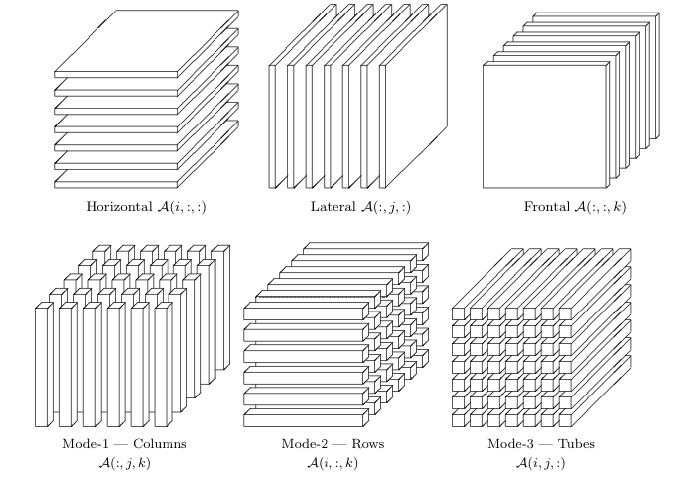
\includegraphics[width=0.9\textwidth]{slicesoftensors}
  \caption{Slices and Fibers of tensors}\label{fig:slicesoftensors}
\end{figure}

\begin{figure}[H]
  \centering
  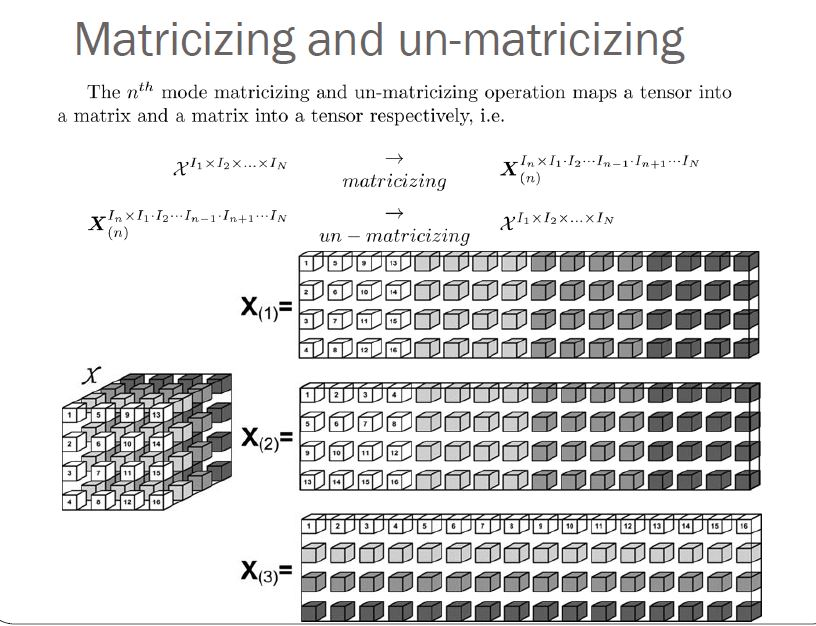
\includegraphics[width=0.9\textwidth]{matrizeandunmatrize}
\end{figure}

The N-mode multiplication of an order $N$ tensor $\mathcal{X}^{I_1 \times I_2 \times ... \times I_n}$ with a matrix $M^{J \times I_n}$ is given by

\[
    \mathcal{X} \times_n \bm{M} = \mathcal{X} \bullet_n \bm{M} = \mathcal{Z}^{I_1 \times I_{n-1} \times J{n} \times I_n + 1 \times ... \times I_n}
\]

Where

So this operation is given by

\[
    [\mathcal{X} \times_n \bf{M}]_{(n)} = \bf{M}\bf{X}_{(n)}
\]

For we have the SVD as n-mode multiplication

Notation generalizes matrix-matrix products:

\begin{align*}
  \bf{A} \times_1 \bf{U} & = \bf{U}\bf{A} \\
  \bf{A} \times_2 \bf{V} & = \bf{A}\bf{V}^T \\
  \bf{A} = \bf{U}\Sigma\bf{V}^T & = \Sigma \times_1 \bf{U} \times_2 \bf{V}
\end{align*}

Can express matrix SVD with n-mode products

\begin{figure}[H]
  \centering
  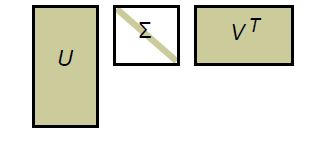
\includegraphics[width=0.9\textwidth]{SVDNmode}
\end{figure}

It is good to know the Kronecker Product. If $\bm{A}$ is an $m \times n$ matrix and $\bm{B}$ is a $p \times q$ matrix then the Kronecker product $\bm{A} \otimes \bm{B}$ is the $mp \times nq$ block matrix

\[
    \bm{A} \otimes \bm{B} =
    \begin{bmatrix}
      a_{11}\bm{B}  & \cdots & a_{1n}\bm{B} \\
      \vdots & \ddots & \vdots \\
      a_{m1}\bm{B} & \cdots & a_{mn}\bm{B}
    \end{bmatrix}
\]

More explicity

\[
    \begin{bmatrix}
   a_{11} b_{11} & a_{11} b_{12} & \cdots & a_{11} b_{1q} &
                   \cdots & \cdots & a_{1n} b_{11} & a_{1n} b_{12} & \cdots & a_{1n} b_{1q} \\
   a_{11} b_{21} & a_{11} b_{22} & \cdots & a_{11} b_{2q} &
                   \cdots & \cdots & a_{1n} b_{21} & a_{1n} b_{22} & \cdots & a_{1n} b_{2q} \\
   \vdots & \vdots & \ddots & \vdots & & & \vdots & \vdots & \ddots & \vdots \\
   a_{11} b_{p1} & a_{11} b_{p2} & \cdots & a_{11} b_{pq} &
                   \cdots & \cdots & a_{1n} b_{p1} & a_{1n} b_{p2} & \cdots & a_{1n} b_{pq} \\
   \vdots & \vdots & & \vdots & \ddots & & \vdots & \vdots & & \vdots \\
   \vdots & \vdots & & \vdots & & \ddots & \vdots & \vdots & & \vdots \\
   a_{m1} b_{11} & a_{m1} b_{12} & \cdots & a_{m1} b_{1q} &
                   \cdots & \cdots & a_{mn} b_{11} & a_{mn} b_{12} & \cdots & a_{mn} b_{1q} \\
   a_{m1} b_{21} & a_{m1} b_{22} & \cdots & a_{m1} b_{2q} &
                   \cdots & \cdots & a_{mn} b_{21} & a_{mn} b_{22} & \cdots & a_{mn} b_{2q} \\
   \vdots & \vdots & \ddots & \vdots & & & \vdots & \vdots & \ddots & \vdots \\
   a_{m1} b_{p1} & a_{m1} b_{p2} & \cdots & a_{m1} b_{pq} &
                   \cdots & \cdots & a_{mn} b_{p1} & a_{mn} b_{p2} & \cdots & a_{mn} b_{pq}
    \end{bmatrix}
\]


and the Khatri-Rao product is

\[
    A = 
    \begin{bmatrix}
      a & b & c \\
      d & e & f
    \end{bmatrix}
\]

\[
    B =
    \begin{bmatrix}
      g & h & i \\
      j & k & l
    \end{bmatrix}
\]


Then $A \odot B$ is the matrix

\[
    A \odot B = 
    \begin{bmatrix}
      ag & bh & ci \\
      aj & bk & cl \\
      dg & eh & fi \\
      dj & ek & fl
    \end{bmatrix}
\]

\section{The Tucker Model}

As seen in lecture \cite[p.~17]{lecture11}

We have the Tucker model. It reads for a third-order tensor $\mathcal{X}^{I \times J \times K}$

\begin{figure}[H]
  \centering
  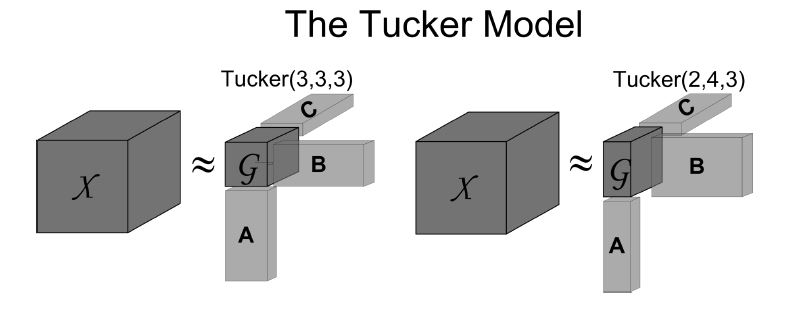
\includegraphics[width=0.9\textwidth]{tuckermodel}
\end{figure}

where the so-called core array $\mathcal{G}^{L \times M \times N}$ accounts for all possible linear interactions between the components of each mode.

The Tucker model is not unique

As a result, the factors of the unconstrained Tucker
model can be constrained orthogonal or orthonormal
(which is useful for compression) without hampering
the reconstruction error. However, imposing orthogonality/
orthonormalty does not resolve the lack
of uniqueness as the solution is still ambiguous to
multiplication by orthogonal/orthonormal matrices $Q$, $R$ and $S$. 

\begin{figure}[H]
  \centering
  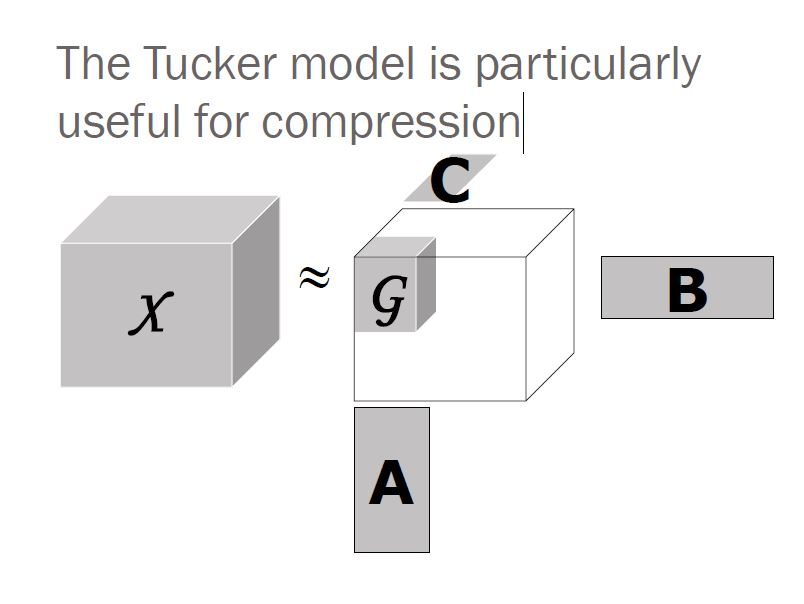
\includegraphics[width=0.9\textwidth]{tuckercompression}
\end{figure}

\section{The CP model}

The CP model can be considered a special case of the Tucker
model where the size of each modality of the core
array $\mathcal{G}$ is the same, i.e., $L = M = N$

\section{Missing Values}

Although methods based on imputation
often are easier to implement (i.e., alternating
least squares can be directly applied), they are
useful only as long as the amount of missing data
is relatively small as their performance tend to degrade
for large amounts of missing data as the intermediate
models used for imputation have increased
risk of convergence to a wrong solution.

Factorizing tensors
based on the CP model have been shown to
recover the true underlying components from noisy
data with up to 99\% data missing for third-order
tensors,40 whereas the corresponding two-way methods
become rather unstable already with 25–40\%
of data missing

 